\section{Results}
\label{sec:results}

\subsection{Failure rates}
\label{sec:results:rates}

\begin{table}[t]
\centering\small
\caption{Per-model results at the medium tier, baseline prompt, task
domains pooled (gpt-4o, gpt-4o-mini and Sonnet~4.6 are HotpotQA only on
the reporting basis). Wilson intervals are computed over attempts, which
are not independent within a run, and are indicative.}
\label{tab:models}
\begin{tabular}{@{}lrrrll@{}}
\toprule
Model & Att. & Fail & Rate & Wilson 95\% & Dominant category (share) \\
\midrule
\code{gpt-5.6-sol} & 255 & 9 & 3.5\% & [1.9, 6.6] & \cat{regex\_pattern} 88.9\% \\
\code{gpt-5.6-luna} & 266 & 11 & 4.1\% & [2.3, 7.3] & \cat{regex\_pattern} 72.7\% \\
\code{claude-opus-4-8} & 265 & 13 & 4.9\% & [2.9, 8.2] & \cat{length\_bound} 76.9\% \\
\code{gpt-5.6-terra} & 266 & 14 & 5.3\% & [3.2, 8.6] & \cat{regex\_pattern} 85.7\% \\
\code{gpt-4o-mini} & 242 & 33 & 13.6\% & [9.9, 18.5] & \cat{regex\_pattern} 66.7\% \\
\code{claude-sonnet-4-6} & 178 & 28 & 15.7\% & [11.1, 21.8] & \cat{length\_bound} 64.3\% \\
\code{gpt-4o} & 250 & 40 & 16.0\% & [12.0, 21.1] & \cat{schema\_mirroring} 72.5\% \\
\code{claude-sonnet-5} & 313 & 67 & 21.4\% & [17.2, 26.3] & \cat{markdown\_wrap} 61.2\% \\
\code{claude-haiku-4-5} & 1{,}329 & 878 & 66.1\% & [63.5, 68.6] & \cat{markdown\_wrap} 72.9\% \\
\bottomrule
\end{tabular}

\end{table}

\Cref{tab:models} gives per-model results. The attempt-weighted failure
rate over the reporting basis is \pn{reported.rate}, but Haiku~4.5
contributes \pn{reported.haiku.failures} of the \pn{reported.failures}
failures. Excluding it gives \pn{reported.exhaiku.rate}, and the
unweighted mean of the nine medium-tier rates is
\pn{reported.medium.macro_rate}. Attempt-weighted aggregates over this
corpus are therefore largely statements about one model, and we report
per-model figures. Rates also mix first attempts with repair attempts,
whose share grows with failure rate; first-attempt validity by node and
per-domain breakdowns are in \cref{app:breakdowns}. No conclusion below
depends on ordering models with similar rates.

\subsection{Dominant-category profiles}
\label{sec:results:profiles}

\begin{figure}[t]
\centering
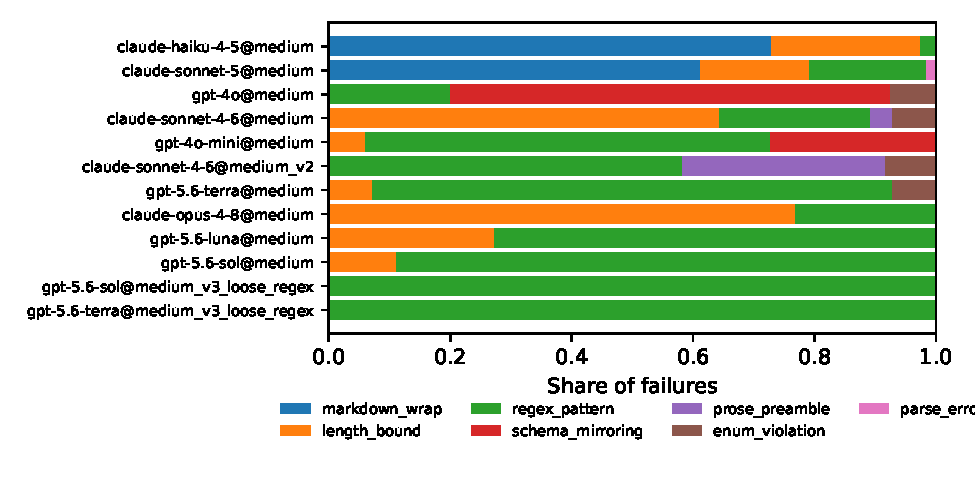
\includegraphics[width=0.92\linewidth]{generated/fig_profiles.pdf}
\caption{Composition of failures by model and schema tier, reporting
basis, ordered by failure rate.}
\label{fig:profiles}
\end{figure}

Grouping models by dominant category gives four observed profiles
(\cref{fig:profiles}): \cat{markdown\_wrap} for Haiku~4.5 and Sonnet~5;
\cat{regex\_pattern} for the three GPT-5.6 models and gpt-4o-mini;
\cat{length\_bound} for Opus~4.8 and Sonnet~4.6; and
\cat{schema\_mirroring} for gpt-4o. These are profiles read off the
dominant category, not clusters from any statistical procedure. They do
not follow vendor tier, since gpt-4o and gpt-4o-mini share a generation
but not a profile, and they do not follow rate: gpt-4o-mini, Sonnet~4.6
and gpt-4o fail at \pn{g.gpt-4o-mini@medium.rate},
\pn{g.claude-sonnet-4-6@medium.rate} and \pn{g.gpt-4o@medium.rate} with
three different dominant categories. Dominant shares for low-rate models
rest on few failures; Opus~4.8's \pn{g.claude-opus-4-8@medium.dominant_share}
share, for example, rests on \pn{g.claude-opus-4-8@medium.failures}
failures (Wilson \pn{g.claude-opus-4-8@medium.dominant_ci}).

Some categories are confined to particular models in our data.
\cat{schema\_mirroring} accounts for \pn{g.gpt-4o@medium.dominant_share}
of gpt-4o failures and was not observed in any GPT-5.6 configuration we
tested. \cat{markdown\_wrap} was not observed for Sonnet~4.6 across
\pn{m.claude-sonnet-4-6.attempts} attempts or Opus~4.8 across
\pn{m.claude-opus-4-8.attempts}, yet it accounts for
\pn{g.claude-sonnet-5@medium.dominant_share} of Sonnet~5 failures and
\pn{g.claude-haiku-4-5@medium.dominant_share} of Haiku~4.5 failures.
Haiku~4.5 and gpt-4o are each dominant in a category the other never
produces. Among the \pn{divergence.groups_qualifying} model--tier groups
with at least 20 failures, the largest difference between two groups in
the share of a single category is \pn{divergence.top.0.pp} percentage
points (\cref{app:divergence}).

\subsection{Profiles depend on the constraint surface}
\label{sec:results:surface}

\begin{table}[t]
\centering\small
\caption{Sonnet~4.6 at the medium and medium\_v2 tiers (HotpotQA). The
cells differ in size and are not paired by question.}
\label{tab:calibration}
\begin{tabular}{@{}lrrrr@{}}
\toprule
& \multicolumn{2}{c}{medium (178 att.)} & \multicolumn{2}{c}{medium\_v2 (324 att.)} \\
\cmidrule(lr){2-3}\cmidrule(lr){4-5}
Category & $n$ & rate & $n$ & rate \\
\midrule
\cat{length\_bound} & 18 & 10.1\% & 0 & 0.0\% \\
\cat{regex\_pattern} & 7 & 3.9\% & 14 & 4.3\% \\
\cat{prose\_preamble} & 1 & 0.6\% & 8 & 2.5\% \\
\cat{enum\_violation} & 2 & 1.1\% & 2 & 0.6\% \\
\midrule
All failures & 28 & 15.7\% & 24 & 7.4\% \\
\bottomrule
\end{tabular}

\end{table}

A profile is not a property of the model alone. Sonnet~4.6 is
\cat{length\_bound}-dominant at the medium tier
(\pn{calib.medium.length_bound} of \pn{calib.medium.failures} failures).
With the caps raised in medium\_v2, \cat{length\_bound} falls to
\pn{calib.medium_v2.length_bound}, \cat{regex\_pattern} becomes dominant
(\pn{calib.medium_v2.regex_pattern} of \pn{calib.medium_v2.failures}), and
the failure rate moves from \pn{calib.medium.rate} to
\pn{calib.medium_v2.rate} (\cref{tab:calibration}).

The error locations identify which caps were binding:
\pn{calib.field.coverage_notes.n} \code{coverage\_notes} values of
\pn{calib.field.coverage_notes.min}--\pn{calib.field.coverage_notes.max}
characters against the 250 cap (mean overrun
\pn{calib.field.coverage_notes.mean_overrun}, maximum
\pn{calib.field.coverage_notes.max_overrun}), \pn{calib.field.answer.n}
\code{answer} values of
\pn{calib.field.answer.min}--\pn{calib.field.answer.max} against 400 (mean
overrun \pn{calib.field.answer.mean_overrun}), and \pn{calib.field.fact.n} \code{fact} value of at most
\pn{calib.field.fact.max} characters against 400. These caps sat below the
lengths the model produced, not far below them. Because medium\_v2 is a
fresh generation, its result could in principle reflect changed output
rather than changed caps. Revalidating the \emph{stored} medium
completions against the medium\_v2 schema, \pn{calib.counterfactual_pass}
of \pn{calib.medium.length_bound} pass, so the elimination is mechanical.

Loosening the identifier character class is the contrasting case. On
HotpotQA, gpt-5.6-sol and gpt-5.6-terra produced
\pn{pert.medium.identifiers} violating identifiers under the baseline
pattern and \pn{pert.medium_v3_loose_regex.identifiers} under the
loosened pattern. Leading-digit violations such as the example in
\cref{sec:intro} went from \pn{pert.medium.leading_digit} to
\pn{pert.medium_v3_loose_regex.leading_digit}, as the loosened class
permits them. Length overflows against the retained 31-character ceiling
occurred under both patterns (\pn{pert.medium.length_overflow} and
\pn{pert.medium_v3_loose_regex.length_overflow}); with a handful of
failures per cell we do not interpret that change or the cell rates
(\cref{app:perturbation}). The relaxation removed the sub-cause it
addressed and did not address length overflow, which the
\cat{regex\_pattern} label conceals because the ceiling is written into
the pattern's quantifier.

\subsection{Formatting failures conceal content failures}
\label{sec:results:concealment}

\begin{table}[t]
\centering\small
\caption{Fence-strip revalidation of \cat{markdown\_wrap} failures,
reporting basis. \emph{Pure formatting} validates once the fence is
removed; \emph{compound} raises a further error.}
\label{tab:fence}
\begin{tabular}{@{}lrrr@{}}
\toprule
Model & Wrapped & Pure formatting & Compound \\
\midrule
\code{claude-haiku-4-5} & 640 & 290 (45.3\%) & 350 (54.7\%) \\
\code{claude-sonnet-5} & 41 & 37 (90.2\%) & 4 (9.8\%) \\
\midrule
All wrapped & 681 & 327 (48.0\%) & 354 (52.0\%) \\
\bottomrule
\end{tabular}

\end{table}

Because \cat{markdown\_wrap} takes precedence, it says nothing about what
lies inside the fence. We stripped the fence from every wrapped failure
and revalidated the payload (\cref{tab:fence}).
\pn{fence.reported.pure_share} validate; the rest raise a further error,
overwhelmingly on length: \pn{fence.reported.concealed.length_bound}
\cat{length\_bound}, \pn{fence.reported.concealed.regex_pattern}
\cat{regex\_pattern} and \pn{fence.reported.concealed.missing_field}
\cat{missing\_field}. The two wrapping models share a dominant category
but not what the wrapper hides: \pn{fence.claude-sonnet-5.compound} of
Sonnet~5's \pn{fence.claude-sonnet-5.n} wrapped failures are compound
(Wilson \pn{fence.claude-sonnet-5.compound_ci}), against
\pn{fence.claude-haiku-4-5.compound_share} of Haiku~4.5's
\pn{fence.claude-haiku-4-5.n}. Counting co-occurrence,
\cat{length\_bound} reaches \pn{reported.length_bound_incl_concealed}
instances against a primary count of \pn{reported.cat.length_bound}, so
primary counts are lower bounds on prevalence.

\begin{table}[t]
\centering\small
\caption{Prompt ablation on Haiku~4.5, HotpotQA, rates over attempts. The
last row counts length violations that are primary or concealed beneath a
fence.}
\label{tab:ablation}
\begin{tabular}{@{}lrrr@{}}
\toprule
& Baseline & Aggressive & Few-shot \\
\midrule
Attempts & 1{,}066 & 189 & 176 \\
\cat{markdown\_wrap} & 49.0\% & 33.9\% & 25.0\% \\
\cat{length\_bound} (primary) & 14.4\% & 16.4\% & 22.7\% \\
\cat{regex\_pattern} & 1.5\% & 2.1\% & 2.3\% \\
Failure rate & 64.9\% & 52.4\% & 50.0\% \\
\midrule
Length violations, primary + concealed & 37.8\% & 30.2\% & 36.9\% \\
\bottomrule
\end{tabular}

\end{table}

Concealment changes how a prompt ablation reads. We ran three
system-prompt variants on Haiku~4.5 on HotpotQA: the baseline, an
aggressive format instruction, and a few-shot prompt
(\cref{tab:ablation}). Wrapping falls from
\pn{ablation.baseline.markdown_wrap} of attempts to
\pn{ablation.few_shot.markdown_wrap}, a relative reduction of
\pn{ablation.delta.markdown_wrap_rel}, and the failure rate from
\pn{ablation.baseline.failure_rate} to \pn{ablation.few_shot.failure_rate}.
Primary \cat{length\_bound} rises from \pn{ablation.baseline.length_bound}
to \pn{ablation.few_shot.length_bound}, which read alone suggests
failures migrating from wrapping to length. But a suppressed fence can
expose a length violation that was already present. Counting primary and
concealed length violations together gives
\pn{ablation.baseline.length_bound_incl_concealed},
\pn{ablation.aggressive.length_bound_incl_concealed} and
\pn{ablation.few_shot.length_bound_incl_concealed}: the combined rate does
not rise as wrapping falls, so the rise in the primary share requires no
increase in over-long output. We do not interpret the differences among
the combined rates, including the lower aggressive figure; the variant
cells are much smaller than the baseline cell, were collected in separate
batches, and are not paired by question.
